\section{基于互信息和局部结构融合的基因调控网络结构推断方法}
\label{sec:locpcacmi}

\subsection{引言}

从基因表达数据中推断基因调控网络~(GRNs)~的结构一直是系统生物学中的十分具有挑战的问题。
鉴定基因之间复杂的调控关系对于理解细胞的调控机制至关重要。
到如今,基于信息理论的各种~GRN~推断方法已经被提出来。
在上一章里面, 我们回顾了各种网络模型和建模方法。
基于信息理论的~GRN~推断方法就是属于关联网络建模方法的范畴。
然而,在传统的DNA~微阵列测序数据中由于存在的外部噪声、
网络结构中的拓扑稀疏性和基因之间的传递依赖等因素,
这些方法在网络推断中会引入假阳性的依赖关系。
特别是随着网络规模的增加,这些推断方法的表现会大幅降低。
在本章节中我们提出了一种新的网络结构推断方法~Loc-PCA-CMI:
首先识别局部重叠基因簇~(local overlapped gene clusters),
然后基于条件互信息~(PCA-CMI)~的路径一致性算法推断每个簇的局部网络结构,
最终通过聚合局部网络结构,也就是基因之间的依赖性网络,来构造最终的~GRN。
我们在~DREAM3~敲除数据集上对~Loc-PCA-CMI~进行了评估,
将其性能与其它基于信息理论的网络结构推断方法,包括~ARACNE、MRNET、PCA-CMI~和~PCA-PMI,进行了比较。
实验结果证明,~Loc-PCA-CMI~在~DREAM3~数据集上特别是在基因数目为~50~和~100~的网络上表现优于其它四种基准方法。

\subsection{相关工作}

推断和理解基因调控网络~(GRNs)~是系统生物学中的一个关键问题, 
可以帮助生物医学科学家明确识别基因与基因之间复杂的调控关系、理解细胞中的调控机制~\cite{altay2010inferring, basso2005reverse}。
在过去,~GRN~是从实验干预中推断出来的,其中基因之间的调控相互作用被验证。
显然,这种方法是不可行的~\cite{elnitski2006locating},需要耗费大量时间和相当大的成本。
由于微阵列技术的发展,大量的基因表达数据通过测序被得到,这使得基于计算方法从这些表达数据中推断出~GRN~成为可能~\cite{maetschke2013supervised}。
% 近年来,基于计算方法的网络推断已成为最重要的目标之一~\cite{altay2010inferring, margolin2006reverse}。
% 已经提出了各种用于GRN推断的方法,例如基于回归的方法~\cite{Huynh-Thu2010, Haury2012, Huynh-Thu2014, liu2014group, li2017mgt, zheng2018bixgboost},
% 基于微分方程的方法~\cite{sakamoto2001inferring, chowdhury2015stochastic, li2011large},
% 贝叶斯和动态贝叶斯网络~\cite{murphy1999modelling, zou2004new, vinh2011globalmit, young2014fast, Liu2016, omranian2016gene},
% 以及基于状态空间的方法~\cite{wu2003modeling, quach2007estimating}。
% 不幸的是,
基因表达数据通常具有高维度和相对较小的样本量,存在``维度诅咒"的问题~\cite{wang2006inferring}。
此外,基因表达数据通常涉及大量外部噪声和非线性关系。
所有这些问题使得准确推断基因之间的调控相互作用,
尤其是在后基因组时代处理大规模基因表达数据时,
变得更加复杂和具有挑战性。

研究者基于各种不同的假设和不同的条件提出了从表达数据构建~GRN~精确结构的各种不同的计算方法~\cite{longabaugh2005computational,karlebach2008modelling}。
目前的这些方法可以大致分为基于模型~(model-based)~和无模型~(model-free)~两大类别。

基于模型的方法通常制定系统的计算模型并进一步学习这种模型的参数。
典型的计算模型包括布尔网络~\cite{shmulevich2002probabilistic,kim2007boolean,bornholdt2008boolean,zhou2016relative},
贝叶斯网络~\cite{kim2003inferring,zou2004new,chen2006effective,needham2007primer,lo2015high},
以及微分方程模型~\cite{gardner2003inferring,di2005chemogenomic,bansal2006inference, honkela2010model,lu2011high,li2011large}。
这些基于模型的方法的细节在上一章中有详细介绍,接下来我们重点介绍基于无模型~(model-free)~的方法。
% 布尔网络模型是最简单的网络模型,它通过布尔变量和布尔逻辑实现。
% 因为基因表达的状态被认为只是活动或非活动,布尔网络模型不能完全捕获复杂的系统行为~\cite{lee2009computational}。
% 贝叶斯网络模型是一种流行的概率图形模型,其中基因之间的依赖关系通过有向无环图描述。
% 贝叶斯网络模型在处理噪声和结合先验知识方面优于其它模型,
% 但该模型中的结构学习是计算密集型的,并且已被证明是~NP~难问题~\cite{chickering2004large}。
% 微分方程模型通过函数表征基因在特定时间的表达水平,其涉及与其它基因的调控相互作用。
% 通常,它将一个基因表达的变化率~(导数)~作为其它相关基因表达水平的函数。
% 使用微分方程模型重建~GRN~的一个主要挑战是如何在高维模型中有效识别模型结构和估计参数。
% 关于各种数据驱动建模方案和相关主题的文章评论,可以参考~\cite{hecker2009gene,marbach2012wisdom,wu2007inference,liu2012reverse,li2018control}。

基于无模型~(model-free)~的方法主要通过衡量基因之间的依赖性来识别调控相互作用,
典型的算法包括基于相关性和基于信息理论的方法。
在基于相关性的方法中,调控相互作用由两个基因之间的共表达程度决定,
例如~Pearson~相关性,秩相关性,欧几里德距离和表达值向量之间的角度~\cite{wang2014review}。
然而,基于相关性的方法无法识别基因之间的复杂依赖性,例如非线性依赖性~\cite{ruyssinck2014nimefi}。
此外,相当多的功能相关基因可能不会共表达,因此难以准确推断调控相互作用。
基于信息理论的方法也是一种具有代表性的无模型~(model-free)~方法,其中互信息~(MI)~有助于衡量基因之间的潜在依赖性,
因为它可以有效地捕获非线性依赖关系~\cite{brunel2010miss,zhang2011inferring}。
近年来,研究者陆续提出了基于信息理论的各种网络推断方法,
其侧重于区分调控中的直接相互作用和间接相互作用~\cite{marbach2010revealing}。

Margolin~等人~\cite{margolin2006aracne}提出了~ARACNE~方法,使用数据处理不等式~(DPI)来过滤掉来自三重基因的间接相互作用。
Meyer~\cite{meyer2007information}~的最小冗余网络~(MRNET)~使用最小冗余特征选择方法~\cite{peng2005feature},
其中对于网络中的每个候选基因,它选择其高度相关基因的子集,同时最小化所选基因之间基于互信息的标准。
Zhang~等人~\cite{zhang2011inferring}~介绍了一种基于条件互信息~(PCA-CMI)~的路径一致性算法; 
Zhao~等人~\cite{zhao2016part}~引入了基于偏互信息~(PCA-PMI)~的路径一致性算法。
路径一致性算法~(PCA,Path Consistency Algorithm)~是一种穷举算法,广泛用于推断~GRN~\cite{zhang2011inferring}。
~PCA-CMI~和~PCA-PMI~这两个算法通常会在运行时间和准确度之间进行折衷权衡。

随着网络规模的增加, 网络噪声本身在增加,
PCA~这种~top-down~的算法的复杂度很高, 而且受到经验参数的影响,使得~GRN~的预测精度急剧下降。
为了改善这种情况,我们直接从局部结构入手,辅助以合并的策略,提出了一种新的基因调控网络结构推断方法,命名为~Loc-PCA-CMI。
该方法首先使用~的高度共同表达的基因作为局部基因簇的质心,
然后用~PCA-CMI~对每个簇的结构进行精炼,~GRN~的最终结构是将所有局部网络结构进行合并。
可以看出,~Loc-PCA-CMI~方法可以处理相对较大的数据集,
并且将从~PCA-CMI~在小规模基因子网的相对准确的结构推断上受益。

\subsection{基于互信息和局部结构融合的基因调控网络结构推断方法~Loc-PCA-CMI}
在本节中,我们将介绍信息理论中的互信息~(MI)~和条件互信息~(CMI)~并简单回顾~PCA-CMI~方法,
然后我们重点介绍提出的~GRN~结构推断方法~Loc-PCA-CMI。

\subsubsection{互信息和条件互信息}
\label{relatedwork}
利用测量两个变量之间的非线性依赖关系时相对高效的优点,
信息理论越来越多地用于衡量基因间的调控关系强弱, 其中互信息和条件互信息应用极为广泛。
互信息~(MI)~的定义如下:
\begin{align} % requires amsmath; align* for no eq. number
    MI(X,Y)=\int \int p(x,y)log \frac{p(x,y)}{p(x)p(y)}dxdy
 \end{align}
 其中~$p(x,y)$~表示两个变量~$X$~和~$Y$~的联合概率密度函数。
~$X$~是基因表达量数据,其中的元素表示不同条件~(样本)~中相应基因的表达值。
~$p(x)$~(或者~$p(y)$)~表示~$X$~(或者~$Y$~)的边缘概率密度分布。

条件互信息~(CMI) 可以用熵表示为:
\begin{equation}
\begin{split}
CMI(X,Y|Z) &= H(X,Z) + H(Y,Z)\\
               & - H(Z) - H(X,Y,Z)
\end{split}
\end{equation}
其中~$H(X,Z)$,~$H(Y,Z)$,~$H(X,Y,Z)$~表示联合熵。
CMI~值越高,表明给定变量~$Z$~,变量~$X$~和~$Y$~之间越可能存在密切关系。

熵可以用高斯核概率密度来估计~\cite{basso2005reverse},变量~$X$~的熵可以通过如下方式计算, 
其中~$|C|$~是变量~$X$~协方差矩阵的行列式~\cite{zhang2011inferring}:
\begin{equation}
    H(X) = log(2\pi e )^\frac{n}{2} |C| ^ {-\frac{1}{2}}
\end{equation}

进一步地,我们可以得到下面的等式:
\begin{equation}
    MI(X,Y)=\frac{1}{2}log\frac{|C(X)|*|C(Y)|}{|C(X,Y)|}
\end{equation}

PCA-CMI~算法利用~MI~和~CMI,从低阶到高阶递归地移除调控网络中具有独立或条件
独立关系的边,其具体步骤如下:

步骤~0:初始化。输入基因的表达数据~$M$, 设置参数~$\beta$~判断独立条件的阈值。
在全部基因的基础上建立全通网络, 并设置~$L=-1$。

步骤~1:$L=L+1$, 对于非零边, $G(i,j) \neq 0$, 选择同时与基因~$i$~和基因~$j$~相连接的邻近基因, 
假定这些基因~(不包括基因~$i$~和基因~$j$~)~的数量为~T。

步骤~2:如果~$T<L$, 停止。如果~$T>L$, 从这~$T$~个基因中选取~$L$~个基因, 
并把它们表示为~$K=[k_1,\ldots,k_L]$。
对于~$K$, 可选择的数目为~$C_T^L$。
对于所有的~$C_T^L$~种~K~,选择计算出~$L$~阶~$CMI(x,j|K)$,
并选择出最大的一个标注为~$I_{max}(x,j|K)$。
如果~$I_{max}(x,j|K) < \beta$, 设~$G(i,j)=0$, 并返回到步骤~1~中。

可以看出~PCA-CMI~是一种采用了~top-down~策略的算法, 
从全通图中不断寻找子图, 在子图的结构里面按照~CMI~的阈值来删减边, 这个独立性的阈值~$\beta$~是全局性的, 
而且需要依靠先验知识来获取。


\subsubsection{Loc-PCA-CMI}

众所周知,生物系统中节点之间是很少完全连通的,
大多数节点只直接连接到少量其它节点~\cite{jeong2000large},因此~GRN~也是一种稀疏网络。
识别网络的稀疏结构的关键步骤是识别可能具有相对高的共表达值的有意义的边。
具体来说,我们提出的方法~Loc-PCA-CMI~首先通过~Pearson~相关分析和~$p$~值错误率~(FDR)~校正选择~top~$n$~条高度共表达的边;
然后, 在缩减的边构成的空间中, 用边连接的基因计算局部重叠基因簇。
然后对于每个局部基因簇, 我们应用~PCA-CMI~算法~\cite{zhang2011inferring},
它可以通过从低到高依赖关联重复去除最可能不相关的边来构建高置信度无向网络~\cite{spirtes2000causation},
直到没有边可以删除,获取每个局部的网络结构~(这个步骤的算法详情见~\ref{relatedwork})。
最后, 我们通过对每个推断的局部子网络结构边权重取平均来获得完整调控网络的最终边的权重。
整个方法流程如图~\ref{pca-cmi-fr}~所示,实现细节如算法~\ref{alg}~所示。
需要注意的是,
在算法~\ref{alg}~里面,
由于~PCA-CMI~本身就非常适合相对较小的~GRN~结构推断,
因此我们设置了一个过滤处理步骤:如果局部类中基因的数量小于或等于常数~$c$,
则直接应用~PCA-CMI~推断~GRN~的结构。
\begin{figure}[!htbp]
    \centering
    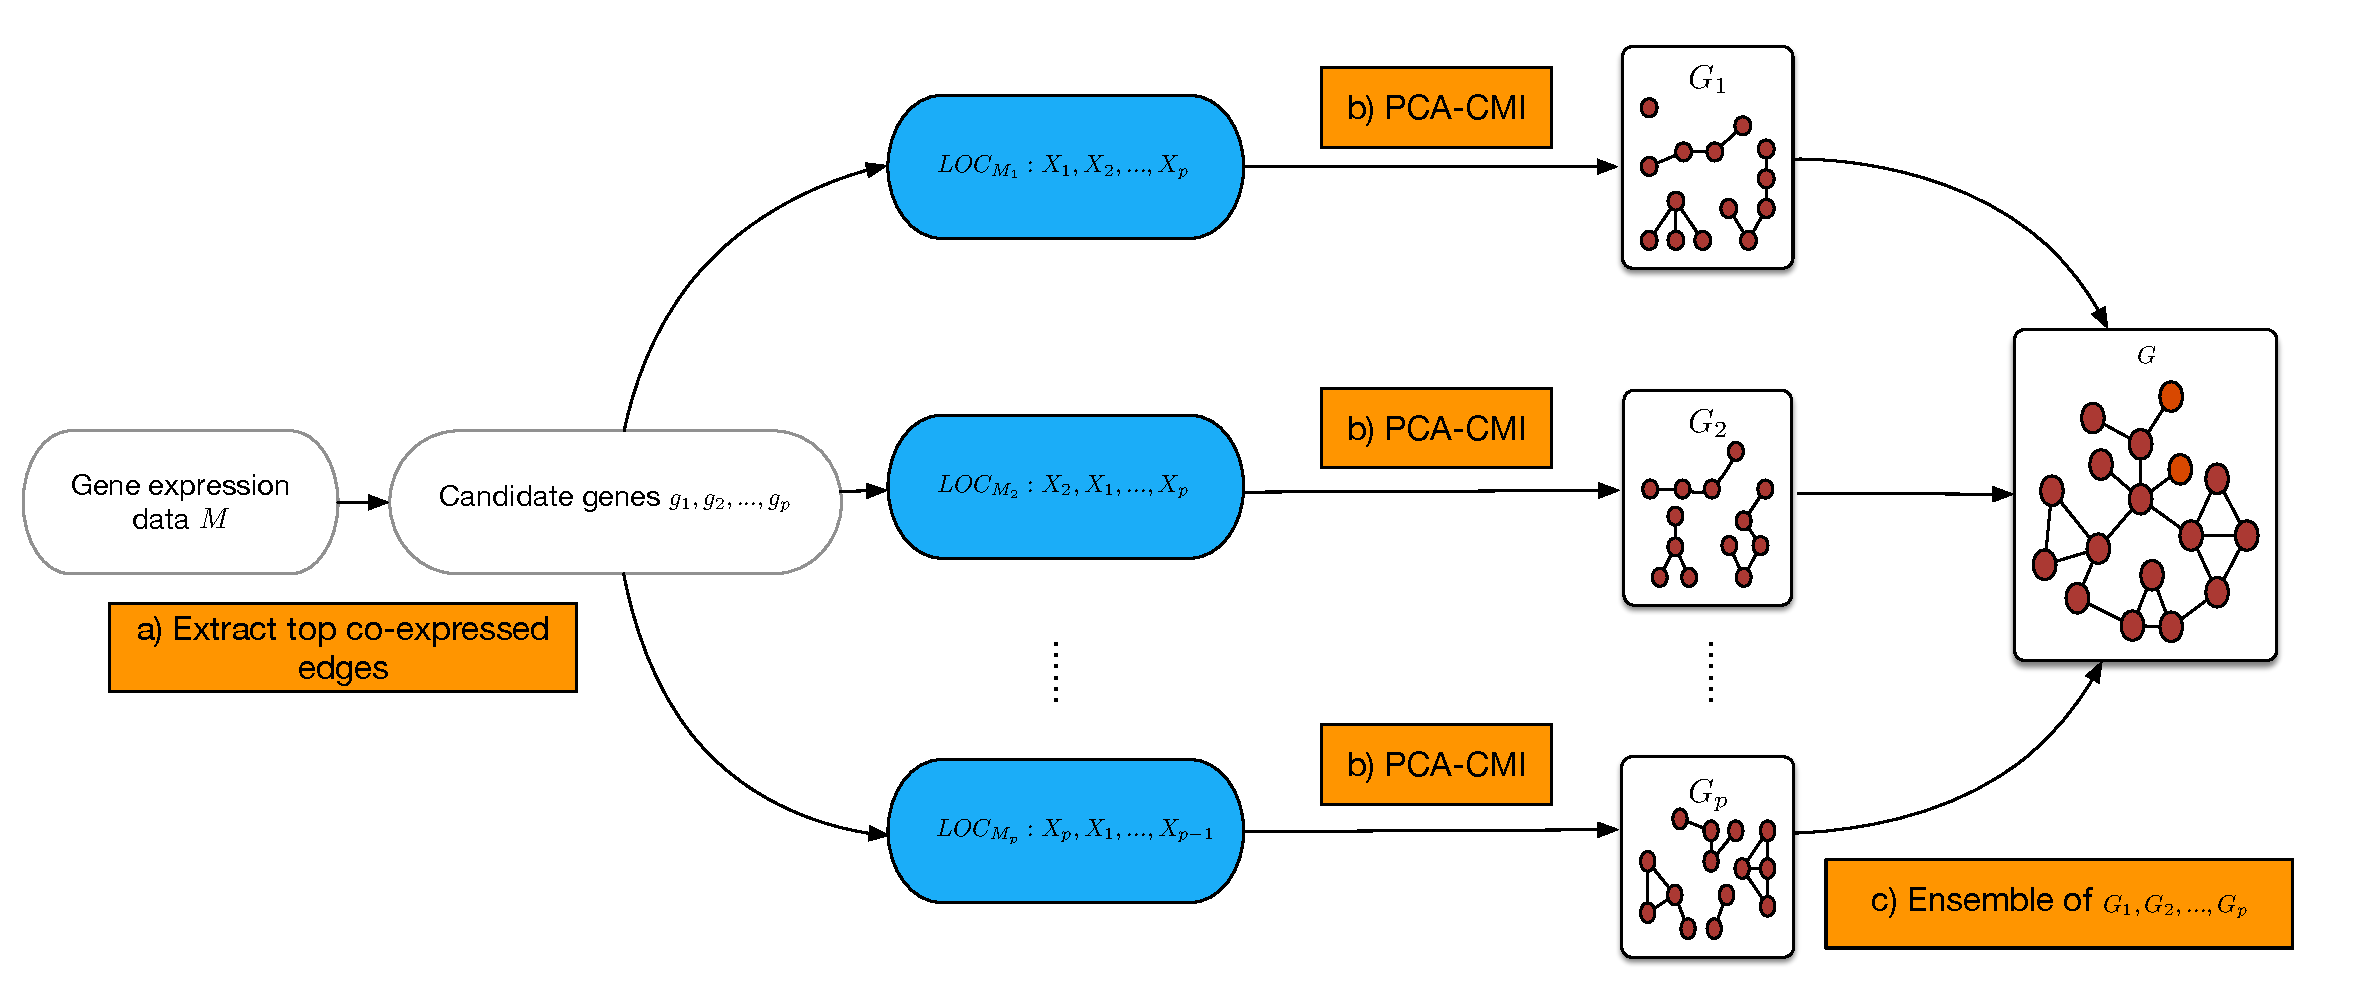
\includegraphics[width=0.95\textwidth]{pca-cmi-framework.pdf}
    \caption{Loc-PCA-CMI~方法框架图.
    (a) 从基因表达矩阵~$M$~中抽取~top~$n$~条共表达边,其对应的候选基因为~$g_1,g_2,\ldots,g_{p}~$。
    这些候选基因被分组到局部簇中~$LOC_{M_1},~LOC_{M_2},\ldots,LOC_{M_{p}}$,
    其中~$g_1,g_2,\ldots,g_{p}$~是分别作为每个簇的质心。
    (b) 对每一个局部之间有重叠的簇,我们应用~PCA-CMI~算法来得到它准确的结构。
    (c) 聚合~$G_1,~G_2,~\ldots,~G_p$~来得到~GRN~的最终结构图~$G$。
    }
    \label{pca-cmi-fr}
\end{figure}



在算法~\ref{alg}~中,在获得每个局部基因簇之后,
~PCA-CMI~和~PCA-PMI~都是后续结构精炼化的候选方法。
除了~Loc-PCA-CMI~外,如果用~PCA-PMI~替换~PCA-CMI,则会生成一种新方法,我们将其命名为~Loc-PCA-PMI。
然后得到四种基于~PCA~(路径一致性)~的方法,即是~PCA-PMI、PCA-CMI、Loc-PCA-PMI~和~Loc-PCA-CMI,
显然所有这些方法都属于无模型~(model-free)~方法。

另外, 如表~\ref{tbl}~所示,在六个基准数据集~DREAM3-10~中,因为~Ecoli~和~Yeast~数据集仅包含~10~个基因,
满足算法~\ref{alg}~的过滤处理条件,
因此~Loc-PCA-CMI~和~PCA-CMI~在这两个数据集上的的表现相同,同理此时~Loc-PCA-PMI~和~PCA-PMI~的表现也会一致。
为了对这些基于~PCA~(路径一致性)~的方法进行有意义的比较,
进一步地,我们选择了其它四个基因数目大于~10~的数据集。

\begin{algorithm}[!htbp]
    \caption{Loc-PCA-CMI~伪代码} %?????
    \label{alg}
    {\bf Input:} %?????? \hspace*{0.02in}??????????? \\ ????
    $M$ (the gene expression data matrix), $m$ (the number of genes), $n$ (the number of top ranked edges), $c$ (constant number); $k$ (CMI order number) and $\beta$ (order threshold) in subroutine PCA-CMI.
    
    {\bf Output:} %???????
    Graph weight matrix $G$ 
    %\begin{spacing}{1.5}
    \begin{algorithmic}[1]
    \If {$m \leq c$} 
    \State $G$ $\leftarrow$ PCA-CMI$(M, k, \beta)$;
    \State \Return $G$
    \Else
    \State Construct pair-wise gene-gene Pearson correlation matrix $\Omega = \rho(M_i, M_j)$;
    \State Select top $n$ edges as $E$ with highest Pearson correlation value in $\Omega$ with FDR correction in p-value, and according to which to get 
    $p$ candidate genes as $g_1,g_2,\ldots,g_{p}$;
    \For{each gene in $g_1,g_2,\ldots,g_{p}$} 
      \State Retrieve its directly connected genes that in edges list $E$ as local cluster $LOC_{M_i}$;
    \EndFor
    \For{each cluster $LOC_{M_i}$  in $LOC$}
      \State $G_{i}$ $\leftarrow$ PCA-CMI$(LOC_{M_i}, k, \beta)$;
    \EndFor
    \State $G$ $\leftarrow$ mean$(G_{1},G_{2},\ldots,G_{p})$;
    \State \Return $G$
    \EndIf
    \end{algorithmic}
    %\end{spacing}
\end{algorithm}

算法~\ref{alg}~的计算复杂度通常由两个参数决定:~第一个是局部重叠基因簇~$p$~的数量,通常低于基因的总体数目~$m$; 第二个是~PCA-CMI~子程序本身的算法复杂度。
~PCA-CMI~的计算复杂度由~CMI~阶数~$k$~和~$LOC_{M_i}$~的簇大小~$|C|$~控制,可以粗略估计为~$O(|C|^k)$~。
因此,~PCA-CMI~的最终算法复杂度为~$O(m *|C|^k)$。
在最坏的情况下, 如果簇大小~$|C|$~等于~$m$, 也就是每个簇包含其中的所有基因, 那么计算复杂度为~$m*m^k = m^{k+1}$。 
然而, 这种最糟糕的情况在实验中很少发生, 因为~$|C|$~通常低于~$m$。
另外, 在实际实验过程中, 所有~PCA-CMI~子程序可以并行执行,~Loc-PCA-CMI~能以很快的速度执行完毕。

\subsection{实验结果}

\subsubsection{数据集}

我们使用来自著名的~DREAM3~竞赛的六个模拟数据~\cite{schaffter2011genenetweaver}~对~Loc-PCA-CMI~的性能进行了基准测试。
~DREAM3~使用~GeneNetWeaver~软件来模拟生成基因网络表达数据,
在来自已知生物模式的调节相互作用系统的子网:~Ecoli~(大肠杆菌)~和~Yeast~(酵母)~的基础上,
得到测试使用的基准网络。 
在实验中,我们采用了~DREAM3~中的总计六个基因敲除表达网络,
其包括三种不同规模的网络节点数:~10、~50、~100, 和两种不同类型的生物:~Ecoli~和~Yeast, 来对所有的测试方法包括~Loc-PCA-CMI~进行评估。

表~\ref{tbl}~展示了这~6~个数据集的详情。
\begin{table} [!htbp]
%\caption{Descriptions of the datasets in our experiments}
\caption{实验所使用的数据集描述} 
\label{tbl} 
\begin{center}
\resizebox{\columnwidth}{!}{%
\begin{tabular} {cccccc} 
\toprule
Datasets  & Number of samples & Average(Max) degree & Number of edges & Network density \\ 
\midrule
DREAM3-10 Ecoli &11 & 2.2(5) & 11 & 0.244\\
DREAM3-50 Ecoli & 51 & 2.48(14) & 62 & 0.051\\
DREAM3-100 Ecoli & 101 & 2.5(14) & 125 & 0.025\\
DREAM3-10 Yeast &11 & 2(4) & 10 & 0.222\\
DREAM3-50 Yeast & 51 & 3.08(13) & 77 & 0.063\\
DREAM3-100 Yeast & 101 & 3.32(10) & 166 & 0.034\\
\bottomrule
\end{tabular}
}
\end{center}
\end{table} 

针对每个数据集而言,输入数据文件中的行代表样本~(实验),~列代表基因~(实验变量)。
第一行是野生型表达数据,该样本中的每个基因都保持稳定状态。
第~$l$~($l>1$)~行则表示在对应的样本中第~$l-1$~个基因敲除后其它基因的表达量。
我们在仓库~\url{https://github.com/chenxofhit/Loc-PCA-CMI.git}~上上传了所有实验所用到的数据集。

\subsubsection{评价指标}

我们通过评估接收者操作特征曲线下面积~(AUROC)~和准确率召回率曲线下面积~(AUPR)~来评估~Loc-PCA-CMI~的性能。
与稀疏生物网络一样,不存在的边~(负样本)~的数量明显超过现有边~(正样本)~的数量; 
事实上,~AUPR~对~AUROC~\cite{saito2015precision}~提供了更多信息。
我们倾向于使用~AUPR~进行评估,但为了与采用~AUROC~作为评估指标的其它方法进行完整地比较,
我们也计算了~AUROC~作为补充。
总体上来讲,较高的~AUROC~和~AUPR~值表明更准确的~GRN~预测。
为此,我们通过比较金标准网络~(golden network)~中的真实边与
方法~Loc-PCA-CMI~输出的有序边列表里最高~$q$~条边来计算真阳性~(TP)、真阴性~(TN)、假阳性~(FP)~和假阴性~(FN)~边的数量。
通过绘制真实阳性率~TPR = TP/(TP + FN)~与假阳性率~FPR = FP/(FP + TN)~来增加~$q$~($q = 1, 2, \ldots, m^2$)~来构建~ROC~曲线。
类似地,通过增加~$q$~来绘制精度~(TP/(TP+FP))~和召回~(TP/TP+FN)~曲线。


\subsubsection{模型选择}
如算法~\ref{alg}~中所述,总计有三个参数会影响方法~Loc-PCA-CMI~的性能。
第一个参数是选定的~top~边的数目~$n$,
如果~$n$~增加,则考虑的共表达的边数目增加,局部基因簇的大小将增加。
第二个参数是~$\beta$,它作为~MI~和~CMI~的阈值来决定独立性。
第三个参数是~CMI~阶数~$k$,从理论上讲,通过增加~$k$,如果~CMI~没有达到~$k-1$~阶的阈值~$\beta$,结构会更准确。
第二个和第三这两个参数也是~PCA-CMI~和~PCA-PMI~里面的参数。
$n$~的最佳值可以通过交叉验证获得,通常较大的~$n$~可以促成使得每个子网络中涵盖更多的基因;
在我们的实验中,我们将其值统一设置为~$n =\binom{m} {2}/5$。
除了上述三个参数外,我们在算法~\ref{alg}~中设置常量~$c = 10$,
即如果基因数小于或等于~10,则~Loc-PCA-CMI~直接调用~PCA-CMI,
显然在这种情况下,~Loc-PCA-CMI~和~PCA-CMI~的性能是相同的。


为了探讨阶数~$k$~的大小是如何影响这些方法的性能,
按照~\cite{zhang2011inferring,zhao2016part}~中建议的参数设置,
设置固定阈值~$\beta = 0.03$~后,
我们把这四种方法中的阶数~$k$~从~1~逐渐变化为~10,
然后分别计算每种方法的~AUROC~和~AUPR。
图~\ref{fig:k}~总结了它们在基准数据集上的结果, 我们可以看出, 阶数~$k$~会对这四种基于~PCA~的方法的结果产生影响,通常当~$k$~达到~4~时~AUPR~和~AUROC~变得稳定,除了~DREAM3-100 Ecoli数据集上略有不同。

\begin{figure*}[!htbp]
    \centering
    \begin{minipage}[b]{0.45\linewidth}
      \centering
      \centerline{
        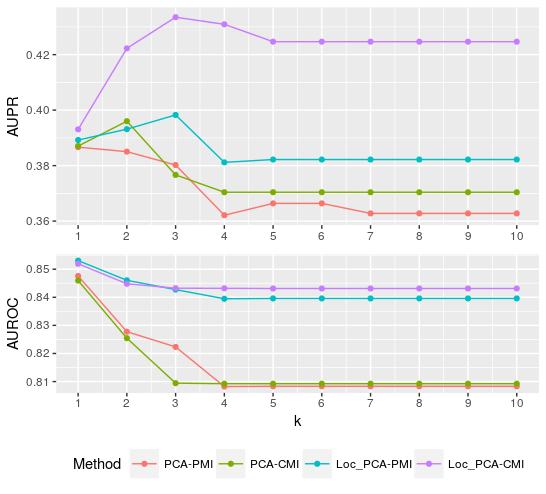
\includegraphics[width = \linewidth]{K_Dream50_Ecoli.png}}
      \centerline{(a) DREAM3-50 Ecoli}
      \medskip  
    \end{minipage}
    \begin{minipage}[b]{0.45\linewidth}
      \centering
      \centerline{
        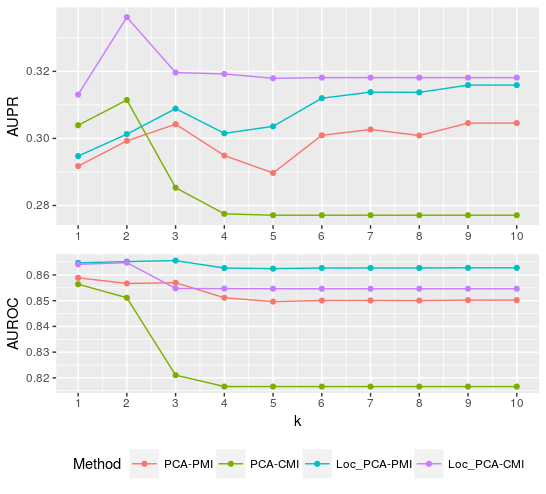
\includegraphics[width =\linewidth]{K_Dream100_Ecoli.png}}
      \centerline{(b) DREAM3-100 Ecoli}
      \medskip  
    \end{minipage}
      \begin{minipage}[b]{0.45\linewidth}
      \centering
      \centerline{
        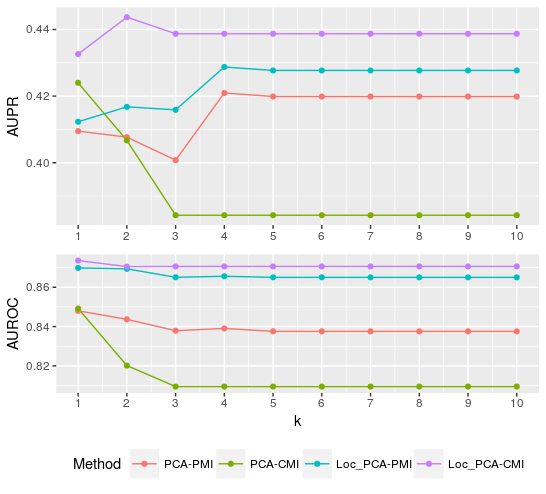
\includegraphics[width = \linewidth]{K_Dream50_Yeast.png}}
      \centerline{(c) DREAM3-50 Yeast}
      \medskip  
    \end{minipage}
    \begin{minipage}[b]{0.45\linewidth}
      \centering
      \centerline{
        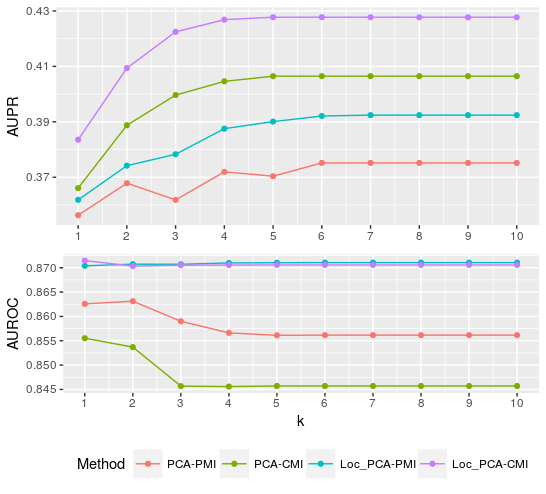
\includegraphics[width =\linewidth]{K_Dream100_Yeast.png}}
      \centerline{(d) DREAM3-100 Yeast}
      \medskip  
    \end{minipage}
    \caption{%AUPR and AUROC  by varying $k$ from 1 to 10 of four PCA based methods on four different datasets: 
    通过在四个不同的数据集上~k~从~1~改变到~10, 基于~PCA~(路径一致性)~的四个算法的~AUPR~和~AUROC~结果示意图。
    }
    \label{fig:k}
    \vspace{-0.5em}
\end{figure*}

固定阶数~$k$=2~后, 我们在~$\beta$=[0.01,0.02,0.03,0.05,0.1,0.15,0.2]~上对这四种算法也进行了测试, 
分别计算出每种方法的~AUROC~和~AUPR。
图~\ref{fig:beta}~总结了它们在基准数据集上的结果, 
我们可以看出, 阈值独立性参数~$\beta$~会对这四种基于~PCA~的方法的结果产生影响,
AUPR~总体上随着~$\beta$~的增加逐渐增大, 然后又逐渐降低。

\begin{figure*}[!htbp]
    \centering
    \begin{minipage}[b]{0.45\linewidth}
      \centering
      \centerline{
        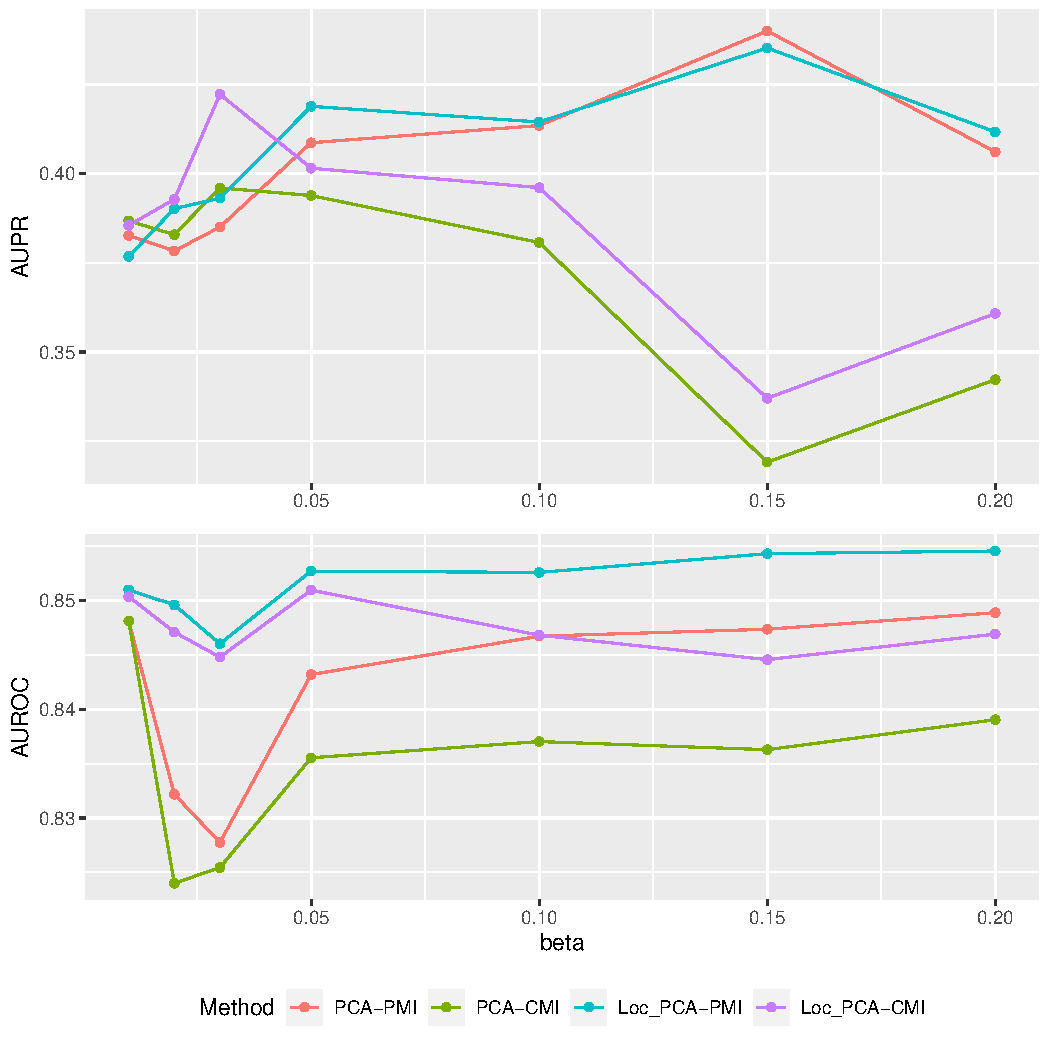
\includegraphics[width = \linewidth]{lamda_Dream50_Ecoli.pdf}}
      \centerline{(a) DREAM3-50 Ecoli}
      \medskip  
    \end{minipage}
    \begin{minipage}[b]{0.45\linewidth}
      \centering
      \centerline{
        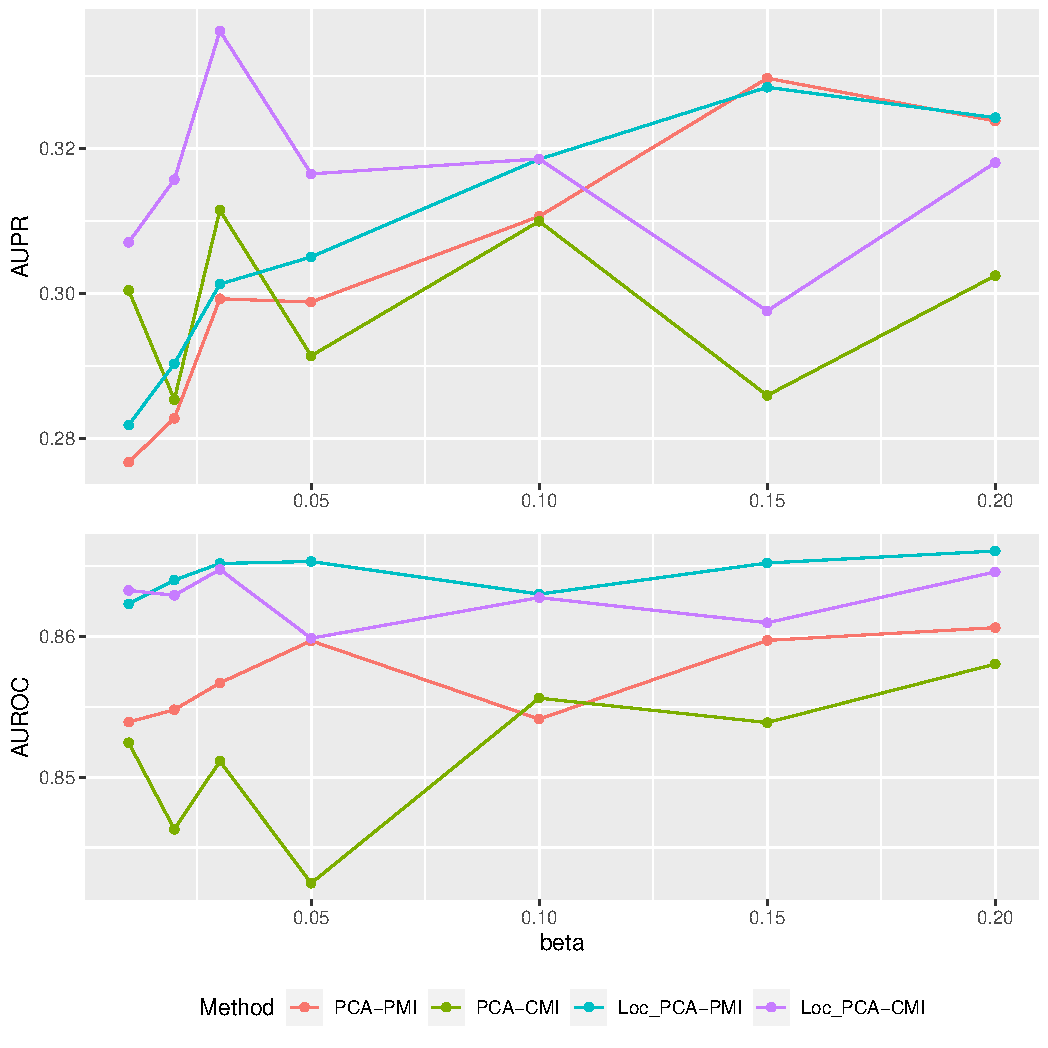
\includegraphics[width =\linewidth]{lamda_Dream100_Ecoli.pdf}}
      \centerline{(b) DREAM3-100 Ecoli}
      \medskip  
    \end{minipage}
      \begin{minipage}[b]{0.45\linewidth}
      \centering
      \centerline{
        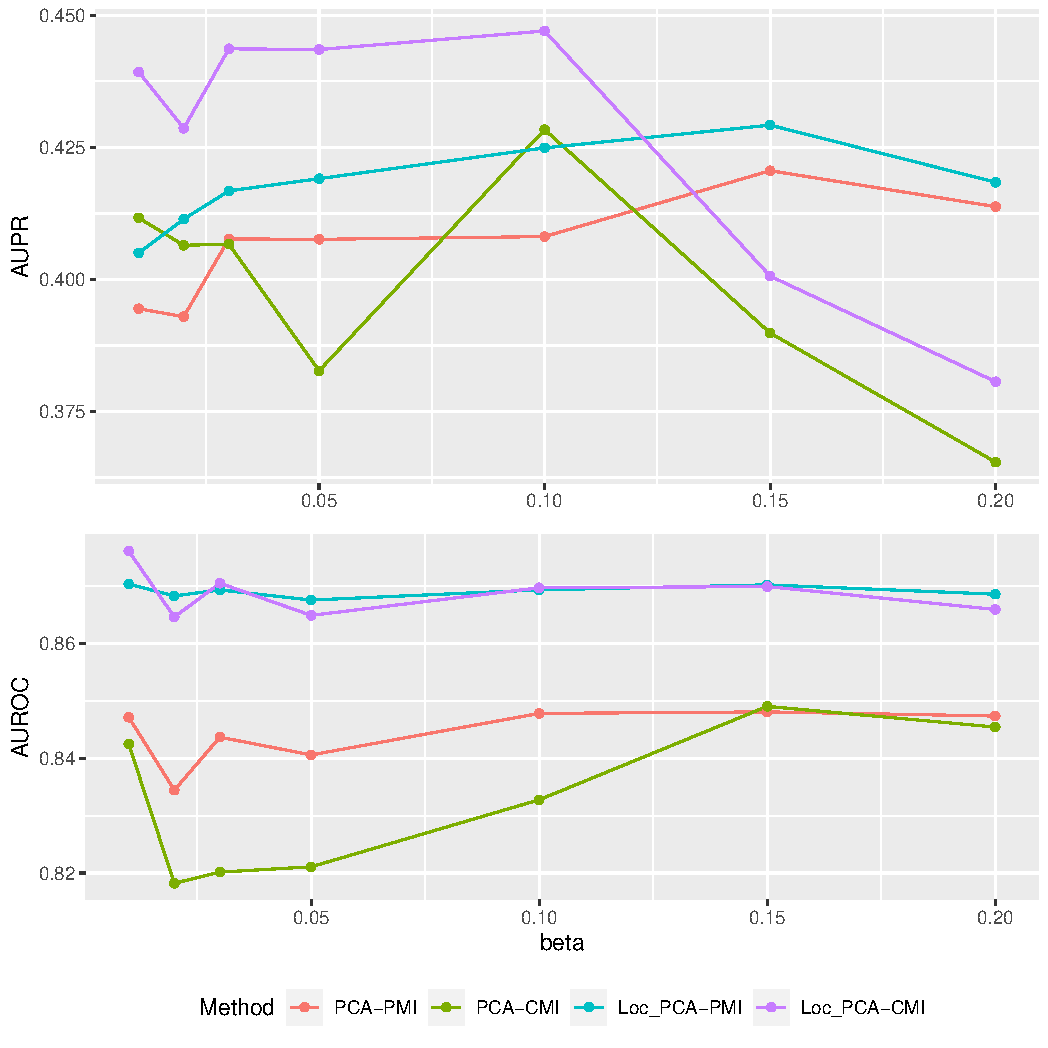
\includegraphics[width = \linewidth]{lamda_Dream50_Yeast.pdf}}
      \centerline{(c) DREAM3-50 Yeast}
      \medskip  
    \end{minipage}
    \begin{minipage}[b]{0.45\linewidth}
      \centering
      \centerline{
        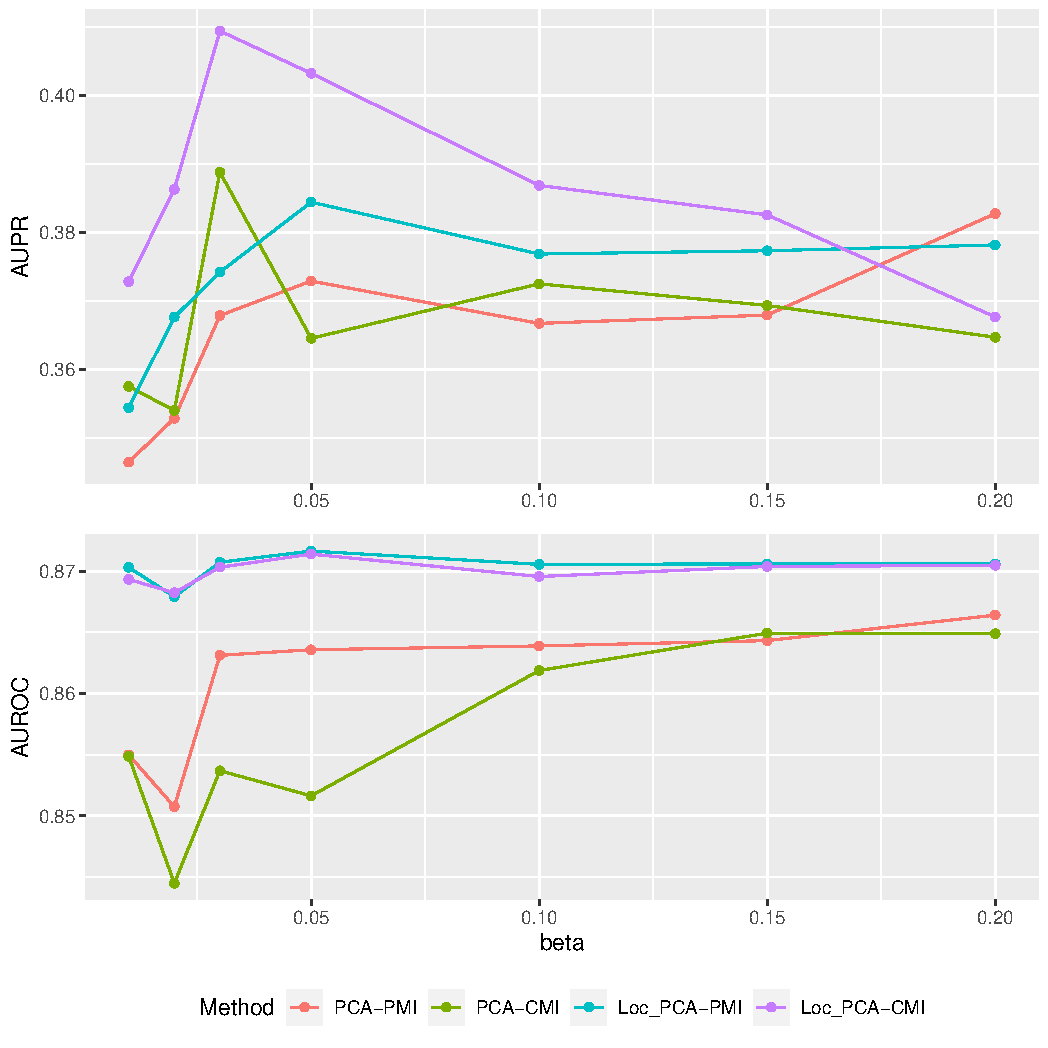
\includegraphics[width =\linewidth]{lamda_Dream100_Yeast.pdf}}
      \centerline{(d) DREAM3-100 Yeast}
      \medskip  
    \end{minipage}
    \caption{%AUPR and AUROC  by varying $k$ from 1 to 10 of four PCA based methods on four different datasets: 
    通过在四个不同的数据集上~$\beta$~逐步改变, 基于~PCA~(路径一致性)~的四个算法的~AUPR~和~AUROC~结果示意图。
    }
    \label{fig:beta}
    \vspace{-0.5em}
\end{figure*}

\subsubsection{实验结果分析}
%\subsubsection{局部结构策略的引入有效提升了~PCA-CMI~和~PCA-PMI~的性能}

相对于~PCA-CMI, ~Loc~PCA-CMI~引入了
根据共表达的边进行局部基因聚类的策略, 为了验证这个策略是否有效, 我们对比了~Loc~PCA-CMI~和~PCA-CMI~在~AUPR~上的变化。
同理, 我们也对比了~Loc~PCA-PMI~和~PCA-PMI。
这四个算法的参数统一设置为:~$\beta = 0.03$,~$k = 2$。
结果如图~\ref{fig:loc}~所示,
在这四个不同的数据集上,~Loc-PCA-CMI~和~Loc-PCA-PMI~分别比~PCA-CMI~和~PCA-PMI~具有更高的~AUPR~值,
可以看出局部聚类策略有助于提高方法~PCA-CMI~和~PCA-PMI~的性能。

\begin{figure*}[!htbp]
  \centering
  \begin{minipage}[b]{0.45\linewidth}
    \centering
    \centerline{
      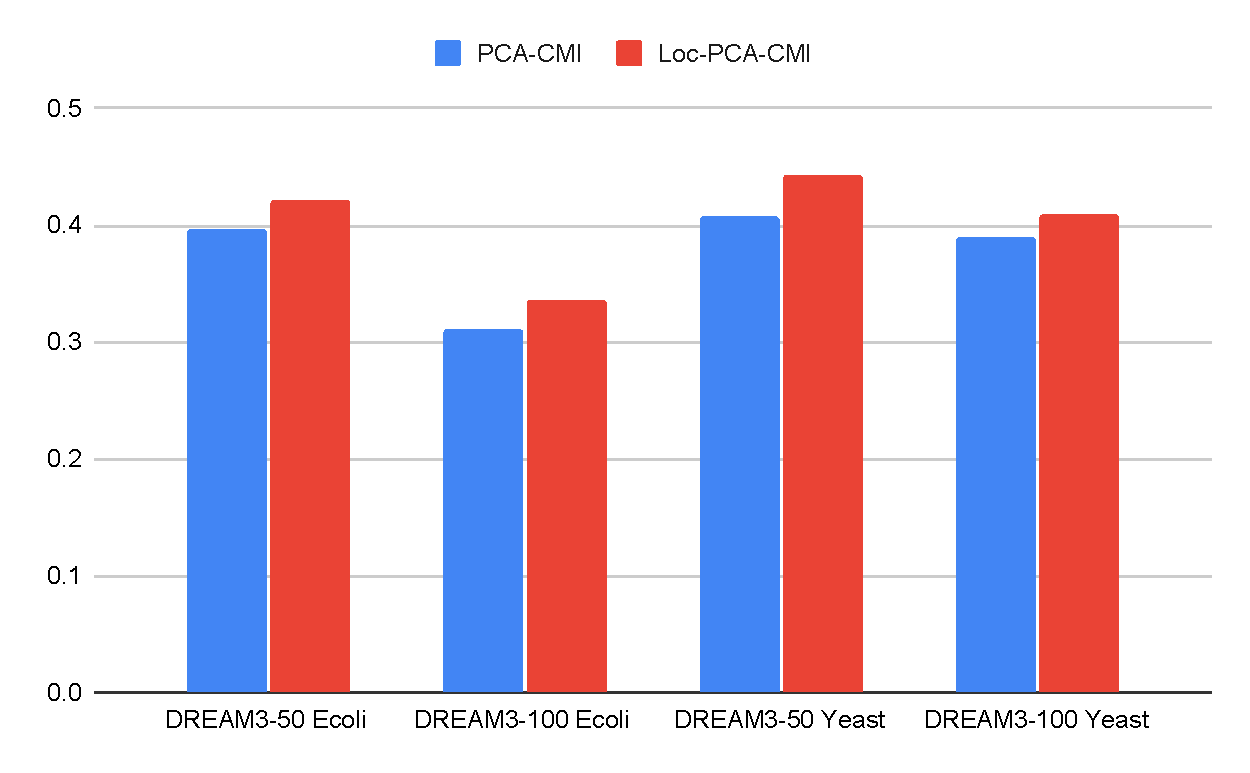
\includegraphics[width = \linewidth]{chart_loc_pcacmi_aupr.pdf}}
    \centerline{(a)~Loc-PCA-CMI~和~PCA-CMI}
    \medskip  
  \end{minipage}
  \begin{minipage}[b]{0.45\linewidth}
    \centering
    \centerline{
      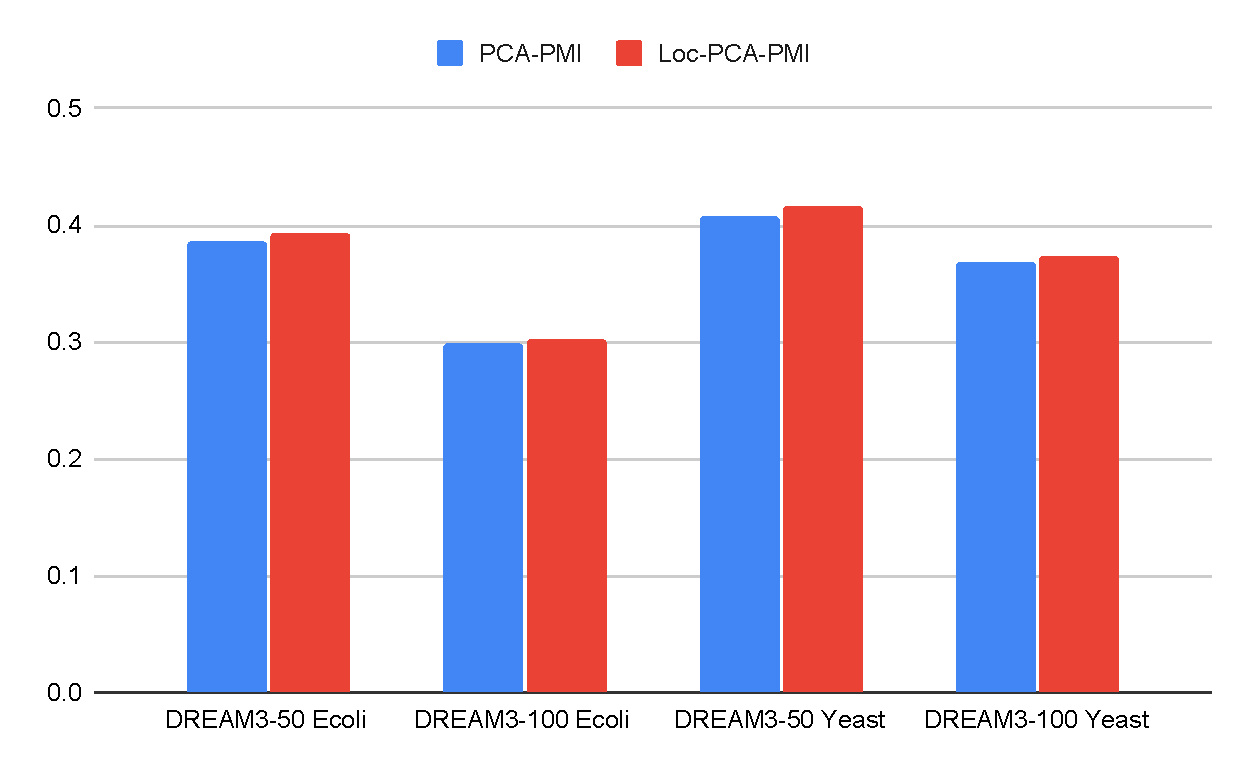
\includegraphics[width =\linewidth]{chart_loc_pcapmi_aupr.pdf}}
    \centerline{(b)~Loc-PCA-PMI~和~PCA-PMI}
    \medskip  
  \end{minipage}
    
  \caption{
    局部结构策略的引入提升了~PCA-CMI~和~PCA-PMI~的性能。
  }
  \label{fig:loc}
  \vspace{-0.5em}
\end{figure*}

% \subsubsection{Loc-PCA-CMI~比其它竞争方法表现更好}

我们在六个基准数据集上使用~Loc-PCA-CMI~和四种基准方法~ARACNE、MRNET、PCA-PMI、PCA-CMI~进行了比较实验。
我们使用~R~包~``minet"和其默认参数来评估~ARACNE~和~MRNET~\cite{meyer2008minet}。
使用~Pearson~相关系数直接从连续基因敲除表达数据~\cite{olsen2008impact,meyer2010information}~中近似估计方法的~MI~矩阵。
为了实现~PCA-PMI~和~PCA-CMI, 我们根据~\cite{zhang2011inferring,zhao2016part}~中提供的~URL~下载了~MATLAB~代码。
另外,~PCA-PMI~和~PCA-CMI~方法中的参数使用它们推荐的默认值,也就是~$\beta = 0.03$~和~$k = 2$。
对于~Loc-PCA-CMI, 我们还对这两个参数采用了相同的值进行比较。
表~\ref{tab:performance_comparison}~给出了实验结果的~AUROC~和~AUPR。
从表中可以看出,当网络规模增大时, 所有的方法的~AUPR~都会急剧下降。
Loc-PCA-CMI~仅在~DREAM3-10~Yeast~数据集中的~PCA-PMI~(或本章提出的~Loc-PCA-PMI~)之后,
而在其它五个数据集中,就~AUROC~和~AUPR~而言,
Loc-PCA-CMI~表现优于其它四种方法~ARACNE、MRNET、PCA-PMI~和~PCA-CMI。
此外,为了更完整地比较,我们还在表中展示了~Loc-PCA-PMI~的实验结果,
其中~$\beta = 0.03$~和~$k = 2$。
Loc-PCA-CMI~和~Loc-PCA-PMI~在~AUROC~上几乎相同。
然而,在大多数数据集中,~Loc-PCA-CMI~的~AUPR~优于~Loc-PCA-PMI。
我们提供了包括所有方法、基准数据集和测评脚本相关的资料, 
在~\url{https://github.com/chenxofhit/Loc-PCA-CMI.git}~上获取。

\begin{table}[!htbp]

  %\caption{AUROC and AUPR for the six datasets using different methods}  
  \caption{使用不同方法在六个数据集上的~AUROC~和~AUPR~结果}  
  \label{tab:performance_comparison} 
    % \scalebox{0.9}{
    % \begin{minipage}{1.1\linewidth}
    \resizebox{\columnwidth}{!}{%
      \centering  
      \begin{threeparttable}  
        \begin{tabular}{ccccccccccccc}  
        \toprule  
        \multirow{2}{*}{Dataset}&  
        \multicolumn{2}{c}{ARACNE}&\multicolumn{2}{c}{MRNET}&\multicolumn{2}{c}{PCA-PMI}&\multicolumn{2}{c}{Loc-PCA-PMI}&\multicolumn{2}{c}{PCA-CMI}&\multicolumn{2}{c}{Loc-PCA-CMI}\\
        \cmidrule(lr){2-3} \cmidrule(lr){4-5}  \cmidrule(lr){6-7}  \cmidrule(lr){8-9}  \cmidrule(lr){10-11}  \cmidrule(lr){12-13} 
        &AUROC&AUPR &AUROC&AUPR &AUROC&AUPR &AUROC&AUPR &AUROC&AUPR &AUROC&AUPR\\
        \midrule  
        DREAM3-10 Ecoli  & 0.523 &0.255   &0.518&0.258    &0.816&0.483    &0.816&0.483    &{0.825}&{0.499}   &\textbf{0.825}&\textbf{0.499}\\
        DREAM3-50 Ecoli  &0.474 &0.050    &0.529&0.061    &0.828&0.385    &\textbf{0.846}&0.393    &0.825&0.396 &0.845&\textbf{0.422}\\
        DREAM3-100 Ecoli &0.505&0.027     &0.488&0.025    &0.857&0.299    &0.865&0.301    &0.851&0.311       &\textbf{0.865}&\textbf{0.336}\\
    
        DREAM3-10 Yeast  &0.628&0.321     &0.644&0.322    &0.995&0.933    &\textbf{0.995}&\textbf{0.933} &0.993&0.918 &0.993&0.918\\
        DREAM3-50 Yeast  &0.507&0.074     &0.524&0.080    &0.844&0.408    &0.869&0.417 &0.820&0.406   &\textbf{0.871}&\textbf{0.444}\\
        DREAM3-100 Yeast &0.547&0.040     &0.556&0.042    &0.863&0.368    &\textbf{0.871}&0.374 &0.854&0.389   &0.870&\textbf{0.409}\\
        \bottomrule  
        \end{tabular}  
        \end{threeparttable}  
        %   \end{minipage}
        %   }
        }
    \end{table} 

\subsection{讨论和结论}

Loc-PCA-CMI~在处理局部网络结构的时候引入了~PCA-CMI,其计算效率的局限性也会受~PCA-CMI~的限制,
特别是在处理大型数据集时。
因为在大型网络的情况下, 局部基因簇的数量可能会非常大。
但是,如果我们可以控制每个局部簇的大小,我们的方法也将适用于大型数据集。
我们未来的工作之一是改进聚类策略,
例如整合蛋白质复合物~\cite{li2017identification, li2017dynetviewer},
以便更有效地处理大规模样本数据。
另外,值得注意的是,我们主要关注推断~GRN~的结构,并没有考虑网络自身的稳定性问题。
因此,我们未来的研究将尝试从网络稳定性的角度出发推断更鲁棒的基因调控网络结构。

我们从局部基因结构出发, 然后合并局部结构来构造全局网络的想法,提出了一种命名为~Loc-PCA-CMI~的新的基于无模型~(model-free)~的~GRN~结构推断方法。
与~PCA~类算法~top-down~的思想相反,~Loc-PCA-CMI~采用了类似~bottom-up~的策略。
在~DREAM3~敲除数据集上的实验表明,~Loc-PCA-CMI~受益于局部聚类的策略。
此外,~Loc-PCA-CMI~优于其它方法,
包括~ARACNE、MRNET、PCA-PMI~和~PCA-CMI,特别是在大小为~50~和~100~的网络上表现更佳。